
\section{Herangehensweise}
Bereits in der frühen Konzeptphase des Projektes, entschieden wir unsere Arbeit mithilfe des Projektmanagement-Modells nach Scheurer zu organisieren (\textcite{scheurer}). Da dieses umfangreiche Theorie, Werkzeuge und Best Practices für Großprojekte bereitstellt, entschieden wir weiterhin nur die für unser vergleichsweise kleines Softwareprojekt sinnvollen Teile zu implementieren.
In ersten informellen Brainstormings zu grundlegenden Themen wie Spieldesign, Gameplay-Mechaniken, Setting und Technik wurden die groben Rahmenbedingungen der Entwicklung abgesteckt. Diese wurden dann in einer \enquote{Kick-Off}-Veranstaltung konkretisiert und in einer detaillierten Projektsizze festgehalten (im Folgenden zu sehen in den Abbildungen 1 und 2).
%TO-DO: Abbildungen in Anhang + Referenzierungen
\begin{figure}[H]
    \centering
    \caption{Projektsizze vom 27.11.2021}
    \subfloat[][]{\fbox{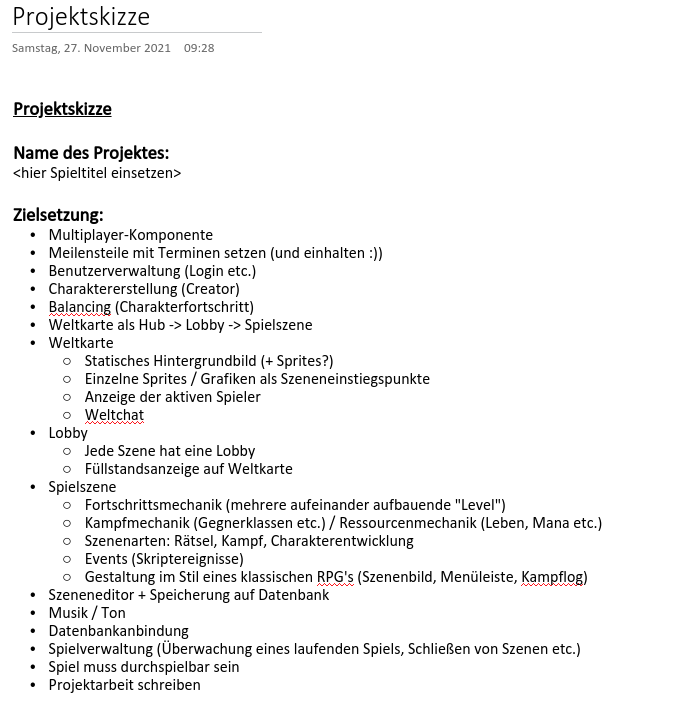
\includegraphics[width=0.5\linewidth]{2021-11-27-projektskizze-1}}}
    \subfloat[][]{\fbox{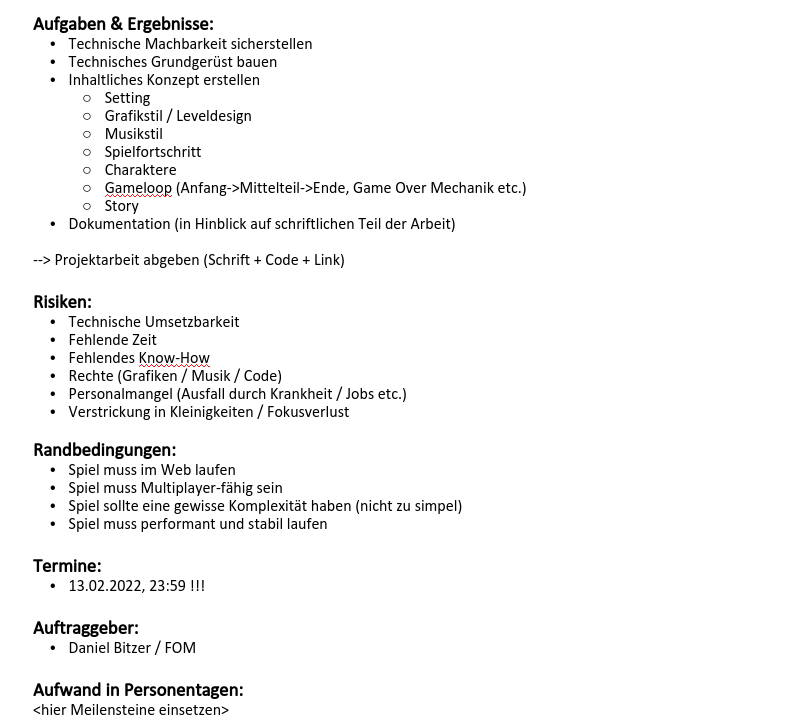
\includegraphics[width=0.5\linewidth]{2021-11-27-projektskizze-2}}}
\end{figure}
%Projektskizze updaten -> Meilensteine rein, nicht realisierte Parts raus
Ziel einer solchen Skizze ist es, einen fokussierten Überblick über alle Aspekte des durchzuführenden Projektes zu gewinnen. Neben allgemeinen Informationen wie Projektname und Auftraggeber, werden Zielsetzung, Aufgaben, erwartete Ergebnisse, Risiken und Randbedingungen definiert. Auch werden wichtige Termine hervorgehoben und Meilensteine für einzelne Teiltätigkeiten gesetzt. Der Definition einer konkreten Zielsetzung kommt hierbei eine herausragende Bedeutung zu, da sich viele der nachfolgenden Aspekte aus eben dieser ergeben. 
\newpage
Den ersten Meilenstein des Projektes stellte die Entwicklung eines rudimentären Prototypen dar, der die technische und konzeptionelle Machbarkeit des Spieles demonstrieren sollte. Darauf aufbauend konnte dann eine (grobe) Aufwandsschätzung erfolgen und es wurden weitere Meilensteine gesetzt.

In Anbetracht unserer eigenen Zielvorstellungen und der im obigen Kapitel erläuterten globalen Anforderungen, entschieden wir das Projekt in drei nebenläufige Teilprojekte zu unterteilen: 
\begin{itemize}
    \item Backend-Entwicklung (Henning Beier)
    \item Frontend-Entwicklung und Grafik-Design (Julian Schäfer)
    \item Game-Design (Rico Pursche)
\end{itemize}

Im Rahmen der \enquote{Backend-Entwicklung} sollte das technische Grundgerüst des Spiels erstellt werden. In diesen Bereich fielen Aufgaben wie die Bereitstellung der Server-Architektur, die Definition und Verwaltung der Datenbank und die Programmierung der Game-Logik.

Im Teilprojekt \enquote{Frontend-Entwicklung und Grafikdesign} lagen die Gestaltung der Website mit HTML, CSS und JavaScript im Fokus. Ein weitere Aufgabe war die Erstellung sämtlicher Grafik-Assets, d.h. Concept Art, Bilder, Sprites, Icons und Animationen.

Setting, Gameplay-Konzept, das Schreiben von Texten, die Ausarbeitung des Kampfsystems und das damit verbundene Balancing lagen im Aufgabenbereich des Teilprojektes \enquote{Game-Design}.

Diese Aufteilung ist hierbei nicht als strikte Trennung zu verstehen, bei der die einzelnen Arbeitsbereiche voneinander abgeschottet sind. Vielmehr wurden Verantwortungsbereiche abgesteckt, die sich auch überschneiden können und das in der Umsetzung auch taten. So wurde häufig in \enquote{teilprojektfremden} Tätigkeitsbereichen gearbeitet, was aber von Beginn an so vorgesehen war. Der Austausch von Daten, Informationen und die Versionsverwaltung wurde über ein gemeinsames Github-Repository realisiert. Änderungen wurden lokal getestet und dann in das Repository geschoben. 

Zudem wurde ein regelmäßiges Meeting am Sonntag eingeplant. Hier wurden der allgemeine Projektstatus besprochen, die Einhaltung der gesetzten Meilensteine überprüft und gemeinsame Entscheidungen über verschiedenste Aspekte des Projektes getroffen.
Ebenfalls wurden Konzepte für Teilthemen wie z.B. Frontend-Layout, Setting und viele Weitere erarbeitet und aufeinander abgestimmt (in den folgenden Abbildungen beispielhaft zu sehen).

%TO-DO: Kampfbildschirm-Layout ordentlich machen und als Grafik einfügen (rudimentär)

\begin{figure}[H]
    \centering
    \caption{Konzept: Kampfsystem vom 29.11.2021}
    \label{fig:2021-11-29-konzept_kampfsystem}
    \fbox{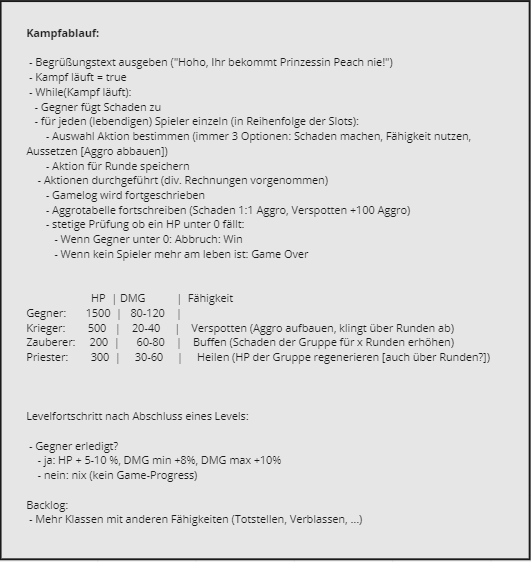
\includegraphics[width=0.7\textwidth]{2021-11-29-konzept_kampfsystem}}
\end{figure}





